%\begin{itemize}
%\item Ahmad Syafrizal Huda (1164062) 
%\item Annisa Fathoroni (1164067) 
%\item Puad Hamdani (1164084) 
%\item Rahmi Roza (1164085) 
%\item Tasya Wiendhyra (1164086) 
%\end{itemize}

\begin{figure}[ht]
\centerline{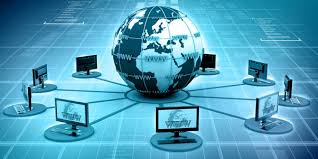
\includegraphics[width=1\textwidth]{figures/1internet.JPG}}
\caption{Internet}
\label{labelgambar}
\end{figure}

\section{Pengertian Internet}
\paragraph{} Pada gambar \ref{labelgambar} merupakan gambar inspirasi tentang internet. Secara harfiah internet adalah kependekan dari interconnected network yang berarti rangkaian komputer yang terhubung satu sama lain. Hubungan melalui suatu sistem antar perangkat komputer untuk lalu lintas data itulah yang dinamakan network. Sebagai contoh yaitu LAN, MAN dan WAN. Misalnya LAN. LAN merupakan singkatan dari Local Area Network yang menghubungkan komputer atau jaringan dalam area tertentu seperti kantor, sekolah atau warnet. Jadi komputer yang terhubung melalui satu jaringan dan saling berkomunikasi dengan waktu dan wilayah yang tidak terbatas, disebut internet.
Internet, sebagai teknologi yang melalui proses pengalihan dari tempat lahirnya ke Indonesia, mengalami proses transformasi dan lokalisasi yang terjadi dalam arena perebutan kekuasaan politik antara negara, korporasi, dan masyarakat sipil. Di dalam arena perebutan kekuasaan ini, titik utama pergulatan ini adalah pembentukan dan penegasan identitas. Berdasarkan pengalaman historis yang ada di Indonesia, tulisan ini mengungkapkan bagaimana internet bersisian dengan pergulatan identitas dan pembentukan komunitas politik yang mandiri di luar negara dan korporasi.
\cite{darma2009buku}.

\section{Sejarah Internet}
\paragraph{} Sejarah Internet : Rangkaian pusat yang membentuk internet diawali pada tahun 1969 oleh ARPA (Advance Research Project Agency), sebuah badan yang dibentuk pada tahun 1958 oleh Amerika yang terdiri dari para peneliti dan teknisi dari universitas dan laboratorium yang ada di Amerika. Awalnya badan ini dibentuk untuk menyaingi Rusia, yang saat itu lebih maju dibidang satelit. Para peneliti bekerja, tidak harus di satu lokasi, untuk membuat penelitian dan mendedikasikan hasil penelitian tersebut untuk perkembangan teknologi Amerika Serikat.

\section{Manfaat Internet}
\begin{table}[h]
\centering
\begin{tabular}{|c|c|}
\hline
Dimensi Kepentingan Penggunaan Internet&Contoh Aktivitas Internet\\
\hline
Informasi&Memperoleh informasi atau berita online\\
Kesenangan&Online untuk alasan yang tidak istimewa,hanya untuk kesenangan atau untuk mnghabiskan waktu\\
komunikasi&Mengirim atau menerima pesan,misalnya email\\
Transaksi&Membeli produk secara online, misalnya buku, musik, mainan atau pakaian\\
\hline
\end{tabular}
\label{table:contoh}
\end{table}
\paragraph{}Pada table \ref{table:contoh} merupakan Klasifikasi Dimensi Kepentingan Penggunaan Internet. Internet di dunia bisnis untuk pergantian informasi, pencatatan produk,media yang mempromosikani, surat elektronik, bulletin boards, kuesioner elektronik, dan mailing list. Biasanya digunakan untuk berkomunikasi,berdiskusi, dan dilibatkan secara proaktif dan interaktif dalam perancangan, pengembangan,pemasaran, dan penjualan produk. Pemasaran melalui internet terdapat 2 metode, yaitu push dan pull marketing. keutamaan dari perencanaan bisnis yang didapat di internet ialah komunikasi dunia dan interaktif diantaranya, serta menyediakan informasi penting dan pelayanan yang sesuai dengan kebutuhan konsumen, juga meningkatkan kerja sama.
\cite{yuliana2004penggunaan}.

\section{Macam-macam Internet}
\subsection{IOT}
\paragraph{} Internet of Things (IOT) merupakan perkembangan keilmuan yang sangat menjanjikan untuk mengoptimalkan kehidupan berdasarkan sensor cerdas dan peralatan pintar yang bekerjasama melalui jaringan internet (Keoh, Kumar, dan Tschofenig, 2014).Menurut (Burange dan Misalkar, 2015) Internet of Things (IOT) adalah struktur di mana objek. orang disediakan dengan identitas eksklusif dan kemampuan untuk pindah data melalui jaringan tanpa memerlukan 2 arah antara manusia ke manusia yaitu sumber ke tujuan atau interaksi manusia ke komputer.
\cite{junaidi2015internet}.
\subsection{ISP}
\paragraph{} Internet Service Provider (ISPs) menghubungkan pengguna dengan perusahaan/pebisnis provider ke internet yang luas atau lebih dikenal dengan internet publik. Para perusahaan ini harus bersaing satu sama lainnya dalam harga, kecepatan, kinerja, dan lainnya. Tetapi mereka pun harus bekerja sama dalam menyediakan konektivitas global dengan semua hal yang berkaitan dengan internet. Tier 1 ISP adalah ISP yang memiliki hak untuk mengakses ke dalam routing internet global tapi tidak membeli transit atau pemberhentian apapun dari orang lain atau pihak lainnya.
\cite{norton2001internet}.
\subsection{Internet Banking}
\paragraph{} Internet Banking ataupun Online Banking didefinisikan sebagai portal dalam internet yang digunakan kostumer untuk melakukan pembayaran, transaksi, untuk berinvestasi. Perkembangan Internet Banking ini dalam hal keuangan dan per bankan membuat cara baru untuk melakukan dan mengatasi permasalahan yang ada pada sehari hari. Penerimaan Internet Banking dalam kalangan masyarakat disambut baik, dan peluasan kontrak e-banking di seluruh dunia saat ini sudah mencapai 50 persen.
\cite{pikkarainen2004consumer}.
\subsection{Cybercrime}
 Cybercrime merupakan kejahatan yang beberapa tahun belakang ini terjadi, media yang digunakan yaitu internet. Kejahatan yang dilakukan beragam, mulai dari mencuri atau mengambil uang dari rekening seseorang, melakukan Bullying, kejahatan seperti menerbitkan video atau pun gambar asusila yang melanggar norma -  norma yang berlaku, sampai menyelundup kedalam properti ataupun jaringan seseorang dan mengakibatkan kerusakan seperti memasukan virus, dan hacking.
\cite{yar2005novelty}.

\section{Pengaruh dan Dampak Internet}
\paragraph{} Pengaruh dan dampak internet sebagai alat media komunikasi. Seperti halnya media massa yang lain, keberadaan internet ini membangkitkan berbagai pertanyaan akan efek negatif yang ditimbulkannya, selain keberadaan efek positif seperti penyampaian dan pengiriman informasi yang cepat dan update melalui fasilitas-fasilitas e-mail, sural kabar online, forum diskusi dan juga chatting serta beragam situs-situs yang ada yang memperkaya khasanah pengetahuan penggunanya. Lebih lanjut keberadaan media komunikasi ini seringkali dianggap sebagai penyebab perilaku asosial penggunanya.
Dampak internet, pemasaran terhadap perusahaan, produk, dan pelayanan menjadi proses yang interaktif saat ini. Situs Web perusahaan bukan hanya sekedar menyajikan katalog produk dan media promosi, melainkan digunakan untuk berdialog, berdiskusi, dan berkonsultasi dengan konsumen secara On-line, bulletin boards, kuesioner elektronik, mailing lists, dan pengiriman surat elektronik. Sehingga semua konsumen dapat dilibatkan secara langsung dalam perancangan, pengembangan, pemasaran, dan penjualan produk.
\cite{surya2009pola}.

\section{Koneksi Ke Internet}
\paragraph{} Ada beberapa macam koneksi yang dapat dilakukan agar anda dapat terkoneksi dengan internet, dan melakukan aktivitas online sepuasnya. Jenis-jenis koneksi juga menentukan kecepatan akses internet anda, dan tentu saja membutuhkan biaya. Perlu diperhatikan pada kecepatan akses, KBps kependekan dari kilobit per second (kilobit per second), yang berbeda dari KBps (kilobyte per second/kilobita per detik), dimana 1 bita sama dengan 8 bit.

\section{Cara Menyimpan Data Ke Internet}
\paragraph{} Ketika mengerjakan file di komputer, membuat sistem back-up, sehingga jika file asli mengalami kerusakan, masih mempunyai file cadangan dan data-data tidak hilang seluruhnya. Memang, bukan berarti membuat Salinan sudah pasti aman, tetap saja ada resikonya, bila semua file di komputer dan flashdisk juga terkena virus. Oleh karena itu, harus memiliki sistem back-up lain. Salah satu cara yang bias dilakukan adalah menyimpannya data di dalam internet.
\cite{lim2014informational}.

\section{Keamanan Internet}
\paragraph{} Untuk melihat keamanan sistem internet perlu diketahui cara kerja internet. Antara lain yang perlu diperhatikan adalah hubungan antara komputer di internet, dan protokol yang digunakan oleh semua orang (public). Untuk mencapai server tujuan, paket informasi harus melalui beberapa sistem yang kemungkinan besar berada di luar kontrol dari kita. Setiap titik yang dilalui memiliki potensi untuk dibobol, disadap, dipalsukan.
\cite{rahardjo2002keamanan}.

\section{Perbedaan Internet dan Media Komunikasi Klasik}
Perbedaan Internet dari media komunikasi klasik dalam penggunaanya:
\begin{itemize}
\item Pengguna internet sebagai perantara untuk berkomunikasi menuntut penggunannya memiliki pengetahuan bagaimana cara menggunakan software baik itu komputer maupun smartphone mereka secara umum dan software aplikasi internet secara khusus.
\item Komunikasi dalam internet selain memiliki konteks komunikasi massa, juga membentuk komunikasi personal dalam jumlah banyak
\item Sifat dan bentuk pesan-pesan yang disampaikan melalui semua media komunikasi dimiliki oleh medium internet
\item Dalam komunikasi melalui internet memungkinkan terjadinya komunikasi antar berbagai personal atau hubungan lain yang memiliki perbedaan, baik itu secara sosiologis maupun budaya.
\end{itemize}
\cite{effendi2009peranan}.

\section{Kelebihan dan Kekurangan Internet}
\subsection{Kelebihan Pada Internet}
    Kelebihan internet sebagai media baru dalam pembelajaran dapat kita lihat sebagai berikut:
\begin{enumerate}
\item Kita bisa menyebarluaskan informasi yang bisa di akses dari mana saja di seluruh dunia dalam waktu singkat.
\item Kita bisa berkomunikasi secara langsung melalui telepon dan unit video processing. Kita bisa melakukan chat melalui jaringan gratis chat yang sangat luas yaitu mIRC.
\end{enumerate}
\subsection{Kekurangan Pada Internet}
    Selanjutnya dapat pula kita lihat kekurangan internet sebagai media baru dalam pembelajaran  sebagai berikut:
\begin{enumerate}
\item Sebagai ajang debat kusir yang berkepanjangan. Ironisnya, debat ini sering kali bersembunyi atas hak anonimitas.
\item Fitnah di era digitalisasi memang menjadi sesuatu yang murah dan diumbar oleh siapa saja tanpa pembuktian yang jelas.
\end{enumerate}
\cite{gafar2017penggunaan}.

